\documentclass{llncs}
\usepackage{hyperref}
\usepackage[utf8]{inputenc}
\usepackage{url}
\usepackage{tikz}
\usetikzlibrary{calc,positioning}
\usetikzlibrary{decorations.text}
\usetikzlibrary{arrows.meta}
\usetikzlibrary{decorations,backgrounds, shapes, shadows}
\usepackage{pgfplots}
\usepackage{amsmath,amsfonts}
\usepackage[stable]{footmisc}
\usepackage{authblk}
\usepackage{xcolor}
\usepackage{graphicx}
\graphicspath{{./Figures/}}
\usepackage[shortlabels]{enumitem}
\usepackage{multicol}
\usepackage{multirow}
\usepackage{comment}
%\usepackage[disable]{todonotes}
\usepackage{todonotes}
\DeclareMathOperator*{\argmax}{argmax}
\DeclareMathOperator*{\argmin}{argmin}
\def\paragraph#1{\subsubsection{#1}}
\def\realWorldInterpretation{\mathcal{R}}
\def\Axioms{\mathcal{A}}
\def\Observations{\mathcal{O}}
\def\logicalModelInstantiation{\Observations2\L}
\def\R{\mathbb{R}}
\def\L{\mathcal{L}}
\def\T{\mathcal{T}}
\def\I{\mathcal{I}}
\def\onto{\textsc{AI4EU-Ontology}}

\def\rb#1{{\color{blue} RAUL: #1}}
\def\cn#1{{\color{red} CHRISTIAN: #1}}
\def\lo#1{{\color{magenta} LUCA: #1}}
\def\jr#1{{\color{purple} JACQUES: #1}}
\def\as#1{{\color{teal} ALESSANDRO: #1}}
\def\jv#1{{\color{violet} JAVIER: #1}}
\def\ps#1{{\color{olive} PETER: #1}}
\def\ls#1{{\color{brown} LUCIANO: #1}}

\title{Foundational aspects of human centered Artificial Intelligence
  in AI4EU}
\author{
Raul Barbosa \inst{1} \and
Luca Iocchi \inst{2} \and
Christian Napoli\inst{3} \and
Jacques Robin\inst{4} \and 
Alessandro Saffiotti\inst{5} \and 
Javier V\'azquez-Salceda\inst{6} \and 
Peter Sch\"uller\inst{7} \and 
Luciano Serafini\inst{8}}

\date{\today}
\institute{
\email{rbarbosa@dei.uc.pt} \and
\email{cnapoli@diag.uniroma1.it} \and
\email{iocchi@diag.uniroma1.it} \and
\email{Jacques.Robin@univ-paris1.fr} \and
\email{alessandro.saffiotti@oru.se} \and
\email{jvazquez@cs.upc.edu} \and 
\email{peter.schueller@tuwien.ac.at} \and 
\email{serafini@fbk.eu} 
}



\begin{document}
\maketitle
\todo{decide the venue}
\todo{invite somebody from Explanable AI}

\begin{abstract}
This paper addresses foundational aspects of \emph{\jr{Human Centered
Artificial Intelligent (HCAI)} agents}, which are physical or software agents, with \jr{AI} components, constructed to interact \jr{or} collaborate with humans.
The article identifies five main concepts that characterise an \jr{HCAI} agent:
\emph{Observation}, \emph{Requirement}, \emph{Action}, \emph{Explanation} and \emph{AI Model}. 
Based upon these, we propose a characterisation of the \jr{qualifiers} of 
\emph{Explainable AI}, \emph{Collaborative AI}, \emph{Verifiable
  AI}, and the relationship between them. 
We focus the analysis on scenarios consisting of a single agent operating in non-deterministic environments
\lo{I would add something like "interacting with people" or "in presence of humans"...}.
\todo{Add a sentence that explains the utility of the contribution of
  this paper.}
Such a characterisation is important for developing AI agents that fulfil their intended function correctly. This requires all artefacts to be amenable to analysis and comprehension by humans, starting from the foundations rather than retrofitted into existing approaches.
\end{abstract}

To propose text modification pleas use the following macros: 
\begin{center}
\begin{tabular}{ll}
the command & will produce \\ \hline 
\verb|\rb{text text text}| & \rb{text text text} \\
\verb|\cn{text text text}| & \cn{text text text} \\
\verb|\lo{text text text}| & \lo{text text text} \\
\verb|\jr{text text text}| & \jr{text text text} \\
\verb|\as{text text text}| & \as{text text text} \\
\verb|\jv{text text text}| & \jv{text text text} \\
\verb|\ps{text text text}| & \ps{text text text} \\
\verb|\ls{text text text}| & \ls{text text text} \\ \hline 
\end{tabular}
\end{center}

To add comment margin comment use the macro 
$$
\verb|\todo{comment comment comment}| 
$$
that produces \todo{comment comment comment}. 

\section{Introduction}

% \paragraph{Agent-Environment pair} 

\lo{I would mention humans immediately in the reference framework, otherwise the human-centered part of the concept will not be clear. What about an agent-human-environment framework? in which human is at the center?}

\as{I agree.  If we propose "foundations for human-centered AI" we should first say what we mean by "human-centerd AI", and then explain why foundations are needed for it.}

\jr{In the definition we can cite the HLEG AI guidelines of Trustworthy AI, https://ec.europa.eu/futurium/en/ai-alliance-consultation/guidelines}

We consider a reference framework composed of an \jr{HCAI} agent (or simply agent) that operates in an
environment \lo{"in presence of humans"...}. We call this framework the agent-environment framework. In an
agent-environment framework there is a clear division between what is
internal to the agent, and what is external to the agent, i.e., the
environment. The agent \jr{observes} the environment via sensors, and \jr{acts upon} 
modifies the environment via \jr{effectors}. Every interaction between the agent
and the environment happens through these two categories. \jr{Observations and actions}
are considered in a very broad sense \todo{observation or percept, not sensors, are the input concepts corresponding to action as output concept. Sensor is the input concept corresponding to the effector input concept}. Sensors range from low level
sensors to input in natural language, images, movies, etc.  Actions
may range from physical actions, as moving ahead, moving an arm,
grasping an object, to communicative actions, such as jr{displaying} some data
on the screen, uttering a sentence, smiling, or playing a song or a
movie. In general
there is no synchronisation between actions and observations, and both
actions and observations can happen independently without following a
precise protocol.  Finally the environment may change due the the effect
of some agent's action, or it may change due to some external cause,
which is not controlled by the agent (e.g., \jr{a human} agent can
operate in the environment) \todo{I took out "some other agent" since the abstract mentions that we restrict the scope of our paper to single agent systems. BTW should we and why? :)}.

% \paragraph{Goal directed agents} 
An AI agent always has one or more goals to achieve\footnote{\jr{The so-called \emph{reflex} agents \cite{aima4}, which internal architecture reduces to a single reasoning component that directly maps observations to actions do not internally maintain an explicit representation of their goals. Even in this case, the mapping function or rule base that implements their reflexes are nevertheless programmed or machine learned with some implicit goal in mind for these agents to achieve.}}. At a given
time-point of its life, some goals can be completely
achieved (and therefore these are not goals anymore), some of them can be
partially achieved, and for other the agent does not have a plan to
achieve them. In order to
achieve its goal(s) an \jr{HCAI} agent can autonomously execute actions \todo{too much content in parentheses, hard to read} (e.g.,
an autonomous agent with a planner obtains these actions by planning)
or some external event may happen so that the agent will get closer to
the goal \todo{Jacques: I do not think this is the best example of "external event" bringing the agent closer to its goal; a simpler, more human-centric example would be \emph{a human collaborating with the agent carries out an action that bring them both closer to their common goal.} (e.g., a classifier is trained with new labelled data)}.
Goals in agents exist on several levels: (i) beneficial properties of
a model and its reasoning on the level of model schema (including
algorithm) design, (ii) high performance (correctness and/or
efficiency) on the level of setting concrete parameters of a model in
an agent, and (iii) goals that are represented within the agent and
direct the agent's behaviour in the world.  Typical machine
learning goals are on level (ii) and typical planning goals are on
level (iii).  However, the agent might have the goal to improve itself
by finding additional data for training (as done in Active Learning)
or by attempting modifications of its own system (similar to genetic
programming) where the levels merge or are all represented within the
agent.

% \begin{tikzpicture}[every node/.style = {scale=.6}]
% \draw (0,0) rectangle (5,3);
% \draw (0,1) -- (4,1) -- (4,2) -- (1,2);
% \node[circle,draw,fill=black!10] (A) at (.5,.5) {A};
% \node[circle,dashed,draw,red,fill=red!10] (G) at (2.5,1.5) {G};
% \foreach \i/\p/\q in {1/1.5/0.5, 
%                      2/2.5/0.5, 
%                      3/3.5/0.5, 
%                      4/4.5/0.5, 
%                      5/4.5/1.5,
%                      6/4.5/2.5,
%                      7/3.5/2.5,
%                      8/2.5/2.5,
%                      9/1.5/2.5,
%                      10/0.5/2.5,
%                      11/0.5/1.5,
%                      12/1.5/1.5}{
% \node[circle,dashed,draw] (\i) at (\p,\q) {A};
% };
% \foreach \i/\j/\a in {A/1/east,
%  1/2/east,2/3/east,3/4/east,4/5/north,5/6/north,6/7/west,7/8/west,8/9/west,9/10/west,10/11/south,11/12/east,12/G/east}
% \draw[->,dashed] (\i) -- node[sloped,above]{\a} (\j);
% \end{tikzpicture}

% \begin{tikzpicture}
% \draw (0,5) -- (0,0) -- (5,0);
% \foreach \i/\n in {0/0.0,1/0.2,2/0.4,3/0.6,4/0.8,5/1.0}{
%    \draw[line width=.1] (-.2,\i) -- (.2,\i);
%    \node at (-.4,\i) {\n};};
% \foreach \i/\n in {0/0.0,1/0.2,2/0.4,3/0.6,4/0.8,5/1.0}{
%    \draw[line width=.1] (\i,-.2) -- (\i,.2);
%    \node at (\i,-.4) {\n};};
% \node[circle,draw,fill=black!10] (C) at (1,1) {C};
% \node[circle,dashed,draw,red,fill=red!10] (G) at (5,5) {C};
% \foreach \i/\p/\q in {1/2/3,
%                      2/4/3.5}{
% \node[circle,dashed,draw] (\i) at (\p,\q) {A};
% };
% \foreach \i/\j in {C/1,1/2,2/G}
% \draw[->,dashed] (\i) -- node[sloped,above]{train} (\j);
% \node[rotate=90] at (-1,2.5) {recall};
% \node at (2.5,-1) {precision};
% \end{tikzpicture}


% \paragraph{Human Centered AI agent} 
\todo{distinguish between the different human roles} 
A way to see human-centered AI is shown in
figure~\ref{fig:hcai-onion}.  An initial observation concerns the fact
that humans cannot be separated from the environment where they
operate. Indeed they are \emph{part} of the environment; they are
\emph{embedded} in it, In other words, humans and environment are
complementary, interconnected, and interdependent in the natural
world, and they interrelate to one another. Therefore Human-Centered Artificial
Intelligence should take into account both humans and the
environment where humans operate.

\begin{figure}[h]
  \begin{center}
    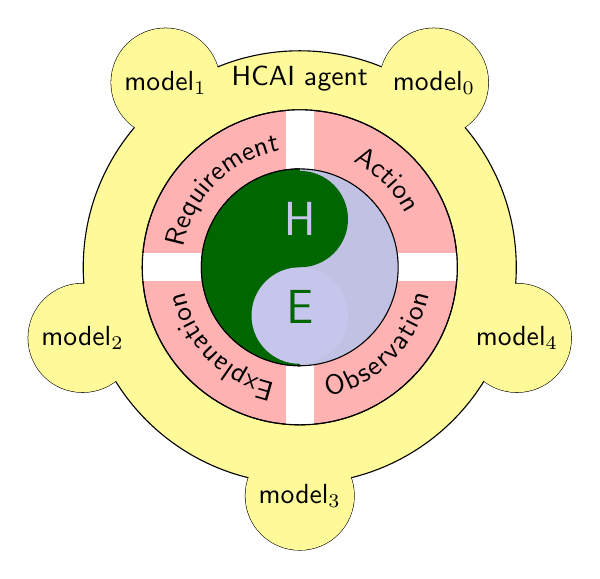
\begin{tikzpicture}\sf
  \foreach \x in {0,...,4}
    \node[draw,circle,fill=yellow!40] at  (\x*360/5+54:2.9) {model$_{\x}$};
  \draw[fill=yellow!40] (0,0) circle [radius=2.75];  
  \draw[fill=red!30] (0,0) circle [radius=2];
  \draw[white,line width=10pt] (-2,0) to (2,0);
  \draw[white,line width=10pt] (0,-2) to (0,2);
  \draw (0,0) circle [radius=2];
  \foreach \x in {1,...,4}
    \coordinate (a\x) at (\x*360/4:1.5);
  \foreach \x in {0,...,4}
    \node[circle,fill=yellow!40] at  (\x*360/5+54:2.9) {model$_{\x}$};
 \node[] at  (90:2.4) {HCAI agent};
    \draw[fill=blue!70!yellow!35] (0,0) circle [radius=1.25];
    \draw[fill=green!40!black] (0,1.25) arc (90:270:1.25);
    \draw[draw=none,fill=green!40!black] (0,.6125) circle [radius=.6125];  
    \draw[draw=none,fill=blue!75!yellow!30] (0,-.6125) circle [radius=.6125];
    \node[circle,fill=green!40!black] at (0,.6125){\color{blue!75!yellow!30}\LARGE H};
    \node[green!40!black] at (0,-.5) {\LARGE E};
  \draw[draw=none,postaction={decorate,decoration={text along path,text align=center,text={Requirement}}}] (a2) to [bend left=45] (a1);
    \draw[draw=none,postaction={decorate,decoration={text along path,text align=center,text={Explanation}}}] (a3) to [bend left=45] (a2);
   \draw[draw=none,postaction={decorate,decoration={raise=-5,text along path,text align=center,text={Observation}}}] (a3) to [bend right=45] (a4);
   \draw[draw=none,postaction={decorate,decoration={text along path,text align=center,text={Action}}}] (a1) to [bend left=45] (a4);

 \end{tikzpicture}

%%% Local Variables:
%%% mode: latex
%%% TeX-master: "main"
%%% End:

\end{center}
\caption{\label{fig:hcai-onion} The Human-Centered Artificial
  Intelligence \cn{I think that we will be required to explain better the figure with a more ``extensive" caption, as well as define human (H) and environment (E). We could change it like that: ``A simple schematization of Human-Centered Artificial Intelligence represented as an set of agents acting as an integrated artificial intelligent systems (external ring) and their interactions (inner ring) with respect to humans (H) and environment (E)"}}
\end{figure}

The external ring in Figure~\ref{fig:hcai-onion} represents the
artificial intelligent agent(s). It can refer to one single
intelligent agent or a set of interrelated intelligent agents, which
autonomously interact following, e.g., a multi-agent paradigm. Every
single artificial intelligent system can implement one (or more) tasks
using one (or more) specific approaches/models. For instance an
``artificial reasoner'' could represent its knowledge in some logical
formalism and support query answering and inference through automatic
reasoning (e.g., SAT, ASP); an ``artificial classifier'' could be
implemented in a deep neural network that is capable to classify
images into different classes. An ``artificial planner'' can produce
plans and take decision exploiting classical planning techniques or
reinforcement learning. To solve complex tasks, different systems and
methodologies should be integrated. A black box integration of each
``intelligent agent'' is not sufficient; it is necessary to integrate
and make all these different approaches to collaborate one another in
a glass-box method. 

Finally, the intermediate ring represents the interaction between the
human/environment and the integrated artificial intelligent system.
The type of interactions that one can see between humans/environment and
artificial agents happen across a set of artifacts that are
``shared'' by the humans/environments and the artificial system.
We briefly describe them here, but we will describe more extensively
in the rest of the document:
\emph{Dependability Requirements} are
artifacts, produced by humans, that specify the expected behaviour and
some other non-functional properties of the artificial intelligent
system. Some of them are usually specified in a formal language (that
has an intuitive semantics for the human) so that it is possible to
verify automatically that the artificial intelligent system behaves
according to the requirement to a certain certainty degree.  Some
of them are not expressed in a formal language and how they can be
represented in a mathematical structure is an open issue.
\emph{Actions} are considered in a broader sense. They
  represent the actions that the artificial agent can perform as well
  as the action that the human can perform in the direction of the
  artificial agent. They can be physical actions (that has effects on
  the environment) or informative actions (that have effects on the
  knowledge of the human or of the artificial agent). 
\emph{Observations} are all the data that the artificial
  intelligent system can collect through its sensors.
\emph{Explanations:} are artifacts that are produced by an artificial
  agent that ``explains'' to the human the reason of its
  behaviour. E.g., the reason why it took an action or a
  decision. Explanations should be human understandable and acceptable
  in a rational system shared by the machine and the human. 



\section{Key concepts of Human Centered AI } 

\subsection{Observations}

% Comments by Sonja:

% This section describes sensors, but mostly sticking to textual examples
% (NLP). There are thousands of types of sensors, and they all serve their
% purpose depending on what data they sense. This is different for all
% pilots - IoT uses variety of sensors: cameras, ultrasonic, infrared,
% etc.; Robotics use potentiometers, accelerometers, Gimbles etc.; Media
% uses cameras.... Perhaps the examples for sensors in this section can be
% specific for each pilot (maybe even include this section in each
% pilot).

% What is the meaning of "sensor of a "text classifier""?  

% Sensor is something that gives information - if this here also stores
% a file, than that is a transducer - does something.

An agent can observe the humans and the environment through its
sensors. Here we mean sensor in a broad sense, i.e., everything that
can be used by the artificial intelligent agent to autonomously
acquire data about the environment (including the humans) and
everything the humans and the environment can use to input data to the
artificial intelligent agent.  Observations are collected via
sensors. There are thousands of types of sensors, and they all serve
their purpose depending on what part of the environment they
sense. Every single pilot in the project has defined a different set
of sensors. E.g., IoT sensors are: cameras, ultrasonic, infrared,
\dots; Robotics sensors are: potentiometers, accelerometers, Gimbles
\dots.; Media sensors include: digital cameras, audio recording,
textual documents, etc.  Essentially, sensor systems are those that
inject input data. Input data can be represented in many different
ways, they can be continuous discrete, structured, lists, trees,
etc. Typically, input data is provided with some meta information that
describes its structure.  Examples of input data are video, picture,
all type of sensors, texts, spoken sentences, etc. In online system,
input data are streams of data, not just a batch of data. Among the
observations we also include the ``commands/requests'' that the human
poses to the artificial agent.  For this reason, one can think that in
general every data is associated with some time stamp $t$ (that can be
relative or absolute). In some cases time information is not relevant
for the decision process of the agent, in other it is. However, what
it should always hold is that agents can take a decision at time $t$
only on the basis of the data that are available to the agent before
this time, i.e., data that are tagged with the timestamp $t'< t$.

Data can be associated with a type and a structure, which should
also be provided as input. 

\begin{definition}
The \emph{observations} of an AI agent are all the data that an agent
can observe at any possible point of its evolution. 
\end{definition}

\subsection{Actions}
\def\actions{\mathcal{A}} Here we consider actions in the very broad
sense as all the possible outcomes of an intelligent system. They can
be physical actions, e.g., the robot is moving 10 cm forward, an
autonomous car braking, an autonomous personal assistant books a room
in hotel Bellavista, or buys 100 stocks of the company SuperGulp.
Actions include also \emph{planning actions}, i.e.  some plan (e.g.,
sequence of simpler actions, or more complex structure of actions) the
agent intends to execute form now on. Another type of action are
\emph{informative actions} that inform the human of a certain
conclusion that the agent has reached. Examples of informative actions
are classifications of input, ranking, predictions done by some
regression model, etc.

In the abstract, any artificial agent can be associated with a set of
actions $\actions$ that it can take. For instance, the set of actions
for a classifier with classes $C_1,\dots,C_n$, is the set
$\{C_1,\dots,C_n\}$ of possible outcome of the classifier. If the
classifier is a multi-classifier, then the set of actions is the set
of all the subsets of $\{C_1,\dots,C_n\}$. If the system is a ranking
system, then its set of actions is the set of ranking functions
of a class of documents provided in input.
The actions associated to a planner that works on a particular
planning domain $\left<S,A,T,s_0,G\right>$ is the set of plans $\pi$
that reaches the goal $G$. The set of actions of a robot that can
navigate a room can be $\{forward(x),turn(\theta) \mid x \in R^+,
\theta \in [-\pi,\pi]\}$.
As one can see from the above example the set of actions associated to
an artificial agent can be discrete or continuous and they strictly
depend from the input.

Notice that in the set of Actions we don't consider the actions
executed by the environment or by the human. As we explained before,
they are part of the Observations.

An important aspect of the actions in human centered AI is that they
should be relevant for the human. For instance in a ranking system,
the user might be interested only in the first 10 documents. In this
case, though the outcome of the system is an entire ranking of all the
documents, the actions which are relevant for the human are only the
first 10 documents in each rank. Another example with physical robots
is the following: the outcome of the planner of a robot could be to
move from the kitchen to the bedroom following one particular path
(path planning) though the human could be interested only in the
starting and ending point of the path, and not in the precise
trajectory that is followed by the robot. Some outcomes of a robot
could also not be perceivable by a human. E.g., the fact that the
personal assistance books the hotel BellaVista through Trivago or
Booking.com is not perceived by the user, which only gets the booking
information as outcome.

\begin{definition}
  The set of actions of an artificial intelligent agent is a set
  $\actions$ which includes all the possible outcomes of the 
  agent that are perceivable and have relevant effects on the human and the
  environment in which the agent operate.
\end{definition}

\subsection{Explanations} 
An explanation is an argument that a human can understand and can
accept. To be understandable the explanation should be given in a
``language'' which is understandable by the human. Furthermore, the
explanation contains an argumentation, (e.g., a sequence of facts and
rules that derives facts from previous facts in the sequence) that
justifies a the conclusion of the artificial agent starting from the
given input. This argument can be a deductive or an inductive
argument. However what is most important is that the human should be
able to decide to accept or not accept such an argument.

In general an explanation of a decision taken by the agent can be
independend from how the agent reaches such a decision. This is
expecially true when the decision is taken by a black-box method such
as a neural network. 

A deductive argument is an argument in which it is thought that the
premises provide a guarantee of the truth of the conclusion. In a
deductive argument, the premises are intended to provide support for
the conclusion that is so strong that, if the premises are true, it
would be impossible for the conclusion to be false.

An inductive argument is an argument in which it is thought that the
premises provide reasons supporting the probable truth of the
conclusion. In an inductive argument, the premises are intended only
to be so strong that, if they are true, then it is unlikely that the
conclusion is false.

In other words in order to define explanation we need to have a
language $L$ and a combination of deductive/inductive $DIS$ system
that are accepted by the human. Within a deductive/inductive system
$DIS$ it is possible to define a set $\Pi$, that called valid
deductions, such that each $\pi$ is a deduction of a decision $A$ from
a set of input data $O$, which is acceptable by the human.

\begin{definition}[Explanation]
  The explanation of a decision/action $A$ of an artificial
  intelligent agent as a reaction of the observations 
  $O$, is an argument in the deductive/inductive system $DIS$
  of the fact that $A$ follows from $O$, i.e., it is a proof $\pi$ of
  $O\models_{DIS} A$
\end{definition}

\subsection{Requirements}
A requirement, or dependability requirement, is an artifact that
describes a set of required behaviors of an artificially intelligent
system. This is central to the problem of verifiable AI, which has the
objective of verifying that the systems meets its dependability
requirements. 
Dependability requirements are expressed in a human understandable
way, they are indeed formulated by humans. Then the problem of
verifiable AI, is how to translate these requirements in algorithms
that verify that the system is compliant with them. 
Being a human produced artifact, providing a sharp definition of
(dependability) requirement is rather complex if not impossible. In
the examples provided in this overview document (e.g., automotive and
medical domain) dependability requirements can be classified into two
categories 
\begin{description}
\item[Input-output constraints for inference:] given a certain (class of) input data
  a specific (class of) output data is required. If input and output
  data classes are described in some logical term then this type of
  requirement can be seen as pairs: 
$$
\Delta\vdash\Gamma 
$$
where $\Delta=\{\delta_1,\dots,\delta_m\}$ is a set of properties of
the input, and $\Gamma=\{\gamma_1,\dots,\gamma_n\}$ is a set of
properties of the expected output. Intuitively $ \Delta\vdash\Gamma $
means that ``if the input meets all the properties in $\Delta$, then
the output should meet at least one property in $\Gamma$.''.  This
input output constraint on inference can also be associated with some
level of satisfiability. E.g., the constraint $\Gamma\vdash\Delta$
should be satisfied at least 99\% of the time.

\item[Input-output constraints for learning:] one of the main
  characteristics of AI systems is that their behaviour is determined
  by the data that are used to train the system. Examples of
  requirement in this sense is the fact that the training data are
  representative of a given population for which the AI system is
  designed. There is no simple way to express this type of requirement
  in some mathematical structure. This could be the subject of further
  study in the project. 
\end{description}



\section{Examples of (classes of) AI Models}
\todo{from model categorization to model use cases}

Providing a complete and coherent classification or even an ontology
of AI models is an ambitious goal,
%
\as{But why should we have such a goal in this paper? (See also my concern at the start of the next Section.)}
%
which probably is not reachable
within the time frame of this projects, however, we believe that an
initial classification is emerging from the AI research community. In
this classification we take a ``technological'' perspective. i.e., we
list different classes on the basis of the set of methodologies which
are used to specify, to represent, and to perform decision within this
model. In particular we will distinguish the following macro classes
of models.


\begin{itemize}
\item \emph{logical models:} the key aspects of the environment and
  the human are represented with a logical theory (set of formulas of
  a logical/formal language) and decision on the basis of this model
  are taken via logical reasoning. Examples of this type of model are
  Logical Knowledge Bases and Ontologies, Logic programs, classical
  planning domains specified via strips or some other action language,
  \dots.  Logical models are specified declaratively with a set of
  terms and formulas from a logic based requirement language. A good
  summary of all different logical models is provided in the book
  \cite{lifschitz2008handbook}. Logical models provide information of
  what is true, what is false and what logically follows from some
  premises.  To have an overview of all the type of models, how they
  can build and how they can used for decision making, planning and
  inference one can refer to the book \cite{minker2012logic}.

\item \emph{probabilistic models:} the key aspects of the environment
  and the human are represented by some probabilistic
  distribution. Decision are taken on the basis of probabilistic
  inference. Examples of this type of models are statistical graphical
  models (e.g., Bayesian networks, hidden Markov models, \dots).
  \begin{quote}
  \it The knowledge and beliefs of
cognitive agents are modeled using probability distributions
defined over structured systems of representation,
such as graphs, generative grammars, or
predicate logic. This development is crucial for making
probabilistic models relevant to cognitive science, where
structured representations are frequently viewed as
theoretically central. Second, the learning and reasoning
processes of cognitive agents are modeled using
advanced mathematical techniques from statistical
estimation, statistical physics, stochastic differential
equations, and information theory
\hfill \cite{chater2006probabilistic}
\end{quote}
Probabilistic models can be specified by directly providing the joint
probability density/mass function of the variables, or via
directed/undirected graphical models. Usually in probabilistic models
there are a set of observable variables (corresponding to the
data/evidences that an agent is capable to observe directly) and a set
of hidden variables, which distribution should be discovered from the
data.

The key concept in this type of model is the \emph{variable assignment},
i.e., an assignment to all the random variables, on which it is
possible to apply the model in order to predict the likelihood of such
an assignment.

\item \emph{Real Functional Models:} the key aspects of the worlds and
  the user are represented through (a set of) real functions that
  take in input observable quantities and produces an estimation of
  some unobservable quantity. Examples of this type of models are
  Linear models, support vector machines, decision trees, random
  forest and (deep) neural networks.

  A large class of ``real function models'' is constituted by neural
  network models. A neural model is a graph of nodes. Each node is
  associated with a non linear activation function, the input of a
  node n is a linear combination of the output of the function
  associated to nodes that precede n. Both the linear combination and
  the activation function are associated with a set of parameters,
  that need to be instantiated in order to fully define the
  function. A neural network model is also associated to a Loss (or
  Cost) function, that determines the approximation error (i.e., difference between known and predicted outputs) to be minimized.
  %LI: replaced "between know values in terms of the input and the  %output values of the network".

  The key concept of a neural network consists in the instantiation of the parameters.
  lo{this is true for all ML models...}

  For every instantiation of its parameters, a neural network
  computes a function $f:R^k\rightarrow R^h$ where $k$ is the number
  of "imput" nodes (i.e., the nodes that don't have any predecessor)
  and h is the number of the output nodes (i.e., the nodes which are
  not predecessor of any other node). The main objective in neural
  network is to find the instantiation of the parameters, that
  minimizes the Loss/Cost function.

\item \emph{Decision models} model the expected advantage an agent
  can obtain in following a certain policy (= action selection
  strategy). The typical reward based model are Markov decision
  models, which constitute the basis of reinforcement learning. The
  key aspect of decision models is the fact that they represent the
  effect of taking actions in terms of reward for an agent. Both in
  reinforcement learning and game theory the main task in this model
  is to produce a policy that maximizes the expected rewards.

\item \emph{Optimization models} An optimization model has three main
  components: (i) An objective function. This is the function that
  needs to be optimized. (ii) A collection of decision variables. The
  solution to the optimization problem is the set of values of the
  decision variables for which the objective function reaches its
  optimal value. (iii) A collection of constraints that restrict the
  values of the decision variables.

\end{itemize}

In many cases a model presents characteristics that are common to
more than one of the classes described above. We call them \emph{hybrid
  models}. Hybrid models are models that attempts to integrate some of
the previous type of models. Examples of such models are approaches
that integrates logical and numerical models (e.g., Logic Tensor
Networks, Lyrics, \dots) approaches that integrate logical and
statistical models (e.g., Markov Logic Networks and Probabilistic
Logic Programming), and finally approaches that integrate numeric,
statistical and logical models (e.g., DeepProbLog, deep probabilistic
logic programming, and Probabilistic Soft Logic)


\section{The lifecycle of AI Models}

In this section we describe the main phases of an AI model. These
phases can be the result of human intervention, automatic 
procedure, or a combination of the two.
\begin{figure}
\begin{center}
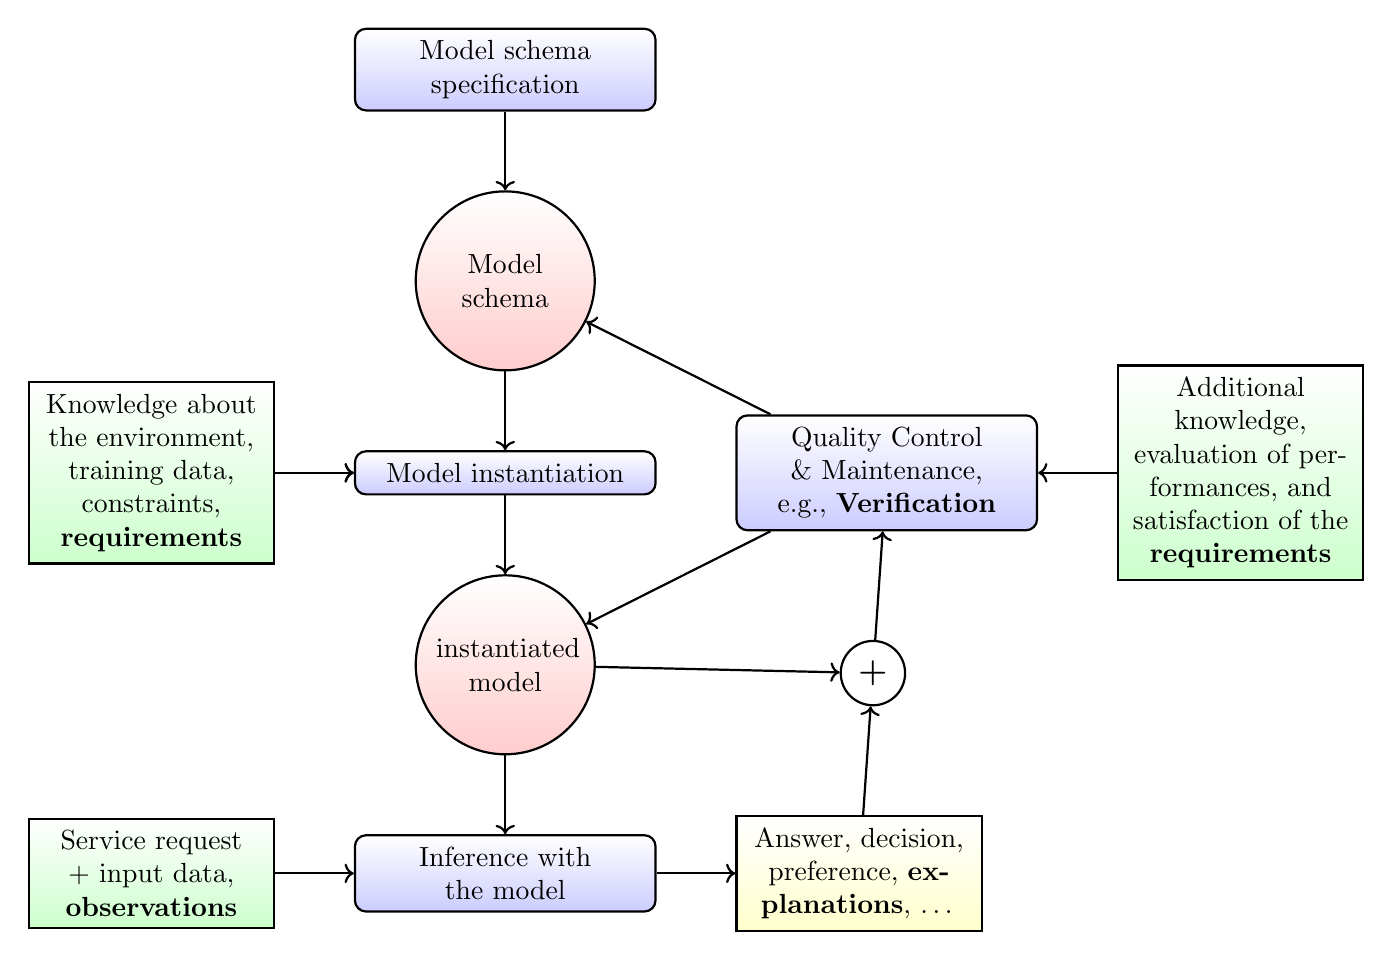
\begin{tikzpicture}[thick,action/.style={shape=rectangle, rounded corners,
                     draw, anchor=center,
                     text width=10em, align=center,
                     top color=white, bottom color=blue!20,
                     inner sep=1ex},
                   model/.style={shape=circle,
                     draw, anchor=center,
                     text width=5em, align=center,
                     top color=white, bottom color=red!20,
                     inner sep=1ex},
            input/.style={shape=rectangle,
                     draw, anchor=center,
                     text width=8em, align=center,
                     top color=white, bottom color=green!20,
                     inner sep=1ex},
            output/.style={shape=rectangle,
                     draw, anchor=center,
                     text width=8em, align=center,
                     top color=white, bottom color=yellow!20,
                     inner sep=1ex}]
 \node[action] (spec) {Model schema specification};
 \node[model,below = of spec] (mschema) {Model schema};
 \node[action,below = of mschema] (inst) {Model instantiation};
 \node[model,below = of inst] (model) {instantiated model};
 \node[action,below = of model] (inference) {Inference with the model};
 \node[action,right = of inst] (revision) {Quality Control \& Maintenance, e.g., \textbf{Verification}};
 \node[input,left = of inst] (knowledge) {Knowledge about the
   environment, training data, constraints, \textbf{requirements}};
 \node[input,left = of inference] (request) {Service request + input
   data, \textbf{observations}};
 \node[input,right = of revision] (add_knowledge) {Additional
   knowledge, evaluation of performances, and satisfaction of the \textbf{requirements}}; 
 \node[output,right = of inference] (answer) {Answer, decision,
   preference, \textbf{explanations}, \dots};
 \node[circle,draw] at ($ (answer) !.5! (revision) $) (plus)
 {\large\bf +};
 \draw[->] (spec) -- (mschema);
 \draw[->] (mschema) -- (inst);
 \draw[->] (knowledge) -- (inst);
 \draw[->] (knowledge) -- (inst);
 \draw[->] (inst) -- (model);
 \draw[->] (model) -- (inference);
 \draw[->] (request) -- (inference);
 \draw[->] (inference) -- (answer);
 \draw[->] (model) -- (plus);
 \draw[->] (answer) -- (plus);
 \draw[->] (plus) -- (revision);
 \draw[->] (add_knowledge) -- (revision);
 \draw[->] (revision) -- (mschema);
 \draw[->] (revision) -- (model);
\end{tikzpicture}
\end{center}
\caption{\label{fig:ai-model-lifecylce} The lifecycle of an artificial
  intelligence model}
\end{figure}

\subsubsection{Model schema specification}

A model schema describes a class of models that shares the same structure. The models within the same class can be obtained by instantiating a (possibly infinite) set of parameters of the model schema (notice that here we use the term parameter in a very broad sense, referring both to the parameters of a probabilistic model, or a neural network, but also to the signature of logical language). Model schema specification is usually done manually, but there is a growing interest in the community in developing methods that (semi-)automatically learn the model structure from a set of observations/data. See for instance structural machine learning, programm sinthesis, non-parametric statistical models, auto-generated neural networks, predicate invention, and learning planning domains.

Associated to a model schema there is also an "intuitive explanation" of part of the models. For instance in choosing a logical lanague to specify the knowledge of an agent, one has to say for some fo the predicates what is the intuitive meaning (i.e., the meaning in the state of the environemt, i.e., the proposition) that is encoded by some predicate. Similarly in a neural network for classifying images in N classes C1,...,CN, one has to say which of the output neuron corresponds to each class Ci.

\subsubsection{Model instance specification/learning/update}

The instantiation of a model schema amounts in setting the "parameters" of the model. This amounts in encoding a certain amount of knowledge about the environment utilizing the "toolset" provided by the model schema. The encoding can be done manually, as often happens in logical rule based models via some knowledge engineering activity, or via supervised learning from data manually tagged by humans with labels, or in a complete unsupervised and automatic manner (e.g., clustering). Statistical models can be obtained by bayesian inference from a set of observations or by Maximum likelihood, or maximum a posteriori inference. Other methods for model specification can also be obtained by "model adaptation" and "transfer learning". Similarly update can be performed automatically via retraining, or manually, by modifying the parameters. Automatic learning of facts and rules from natural language is also possible. Methods for automatic learning of constraints from data are also available

\subsubsection{Inference with the model}
The second important aspect is how the model is used to infer a
decision i.e., an action that the artificial agent decides to
undertake. Given a set of observations $O$ as input, the model
provides as output a set of actions or a policy of actions. This is
obtained by applying an \emph{inference engine} which is defined on
the model.

In this phase the model instance is "queried" about what holds in the
environment. Inference can be very simple (like in neural network,
it's just the computation of the function) or rather complex as for
instance in constraint satisfaction in which it is necessary to apply
seart/optimizaiton algorithms. In logical model inference is done via
some form of logical reasoning (e.g., satisfiability) or model
checking, while in statistical model inference can be a generative
process (generate a data that has certain properties) or to compute
some marginal distribution of a certain (set of) stocastic
variables. What have in common all the above activities is that they
don't change the model they only query it.

\subsubsection{Quality Control and  Maintenance}
%edited by Peter
Once an AI artifact is ready to be used in practice,
additional tasks that are often not part of research activities become important
to reach higher Technology Readiness Levels.

%\begin{itemize}
%\item
For certification purposes and for the permission to use the artifact in practice on/with non-expert users, testing and verification procedures for safety/security-related properties of the behavior of the model can be necessary.
%
%\item
For products that are already in usage and needs to be updated,
maintenance and update methods need to exist so that problems that are identified after shipping the model can be counteracted.
%
%\item
For supporting users and for legal reasons, it can be necessary to have powerful methods for debugging model properties and (re-)actions and for explaining why certain outputs were (or were not) generated. Moreover, in connection with updates of the model, these methods can be useful to prove to authorities that certain behavior is excluded in the future.
%\end{itemize}

This part of the AI artifact lifecycle is very relevant to human-centric artificial intelligence, because it is the longest-lasting process in the existence of the model where the model has contact with a large number of untrained human individuals and unseen input data.


In the following we propose a high level summary of the different
techniques for schema model selection, model specification, learning
and update and inference in the model


\section{Lifecycle for each type of model}

\subsection{Logical models}
  
\paragraph{Formal definition}
A logical langauge $\L$ allows to specify formulas. Formulas are
abstract representation of propositions, i.e., facts that are true or
false in the intended domain. This interpretation is fixed by the
semantics of $\L$ in which is possible to define the class of
\emph{iterpretations} of $\L$. Interpretations are abstract
representations of the state of the enviroment. For every interpretation
$\I$ and every (closed) formula $\phi$ it is possible to predict the
truth value of $\phi$ in $\I$.

A logical model is a set of formulas $\T=\{\phi_1,\dots,\phi_n\}$,
i.e., the facts that are known/believed to be true in the
environment. $\T$ identifies a set of interpretations $\I$ (those
which makes all the formulas in $\T$ true) which are all the possible
situation in which the environment can be according to the agent
knowledge/belief.

The inference task in logical models is satisfiability, i.e, check for
an interpretation $\I$ that satisfies a set of formulas $\T$.

\paragraph{Key concepts}
\begin{description}
\item[logical symbols and relative semantics:] this is the class of
  logical languages schema and the semantics of the logical symbols
  (e.g. classical propositional logic, first order modal fuzzy logic, \
\item[non-logical symbols:] symbols that capture the key aspects of
  the environments (e.g., names for objects, primitive propositions,
  properties, and relations)
\item[logical term:] they denote objects in the environment 
\item[logical formula:] they specify propositions about the state of the
  environemtn
\item[logical interpretation:] specify a state of the environment
\item[satisfiability relation:] $\I\models\phi$ allow to compute the
  truth value of the formulas in a particular interpretation 
\item[logical consequence:] $\Gamma\models\phi$ defines what does it
  mean that the truth value of proposition expressed in the formula
  $\phi$ logically follows from the truth value of a set of
  hypotetical propositions expressed by the formulas in $\Gamma$. 
\end{description}

\paragraph{Model Schema Specification:}
The specification of model is done by choosing: 
\begin{itemize}
\item the set of logical symbols and the relative semantics (i.e.,
  what is usually known as \textbf{the logic}). This choice is usually
  done by the designer and no automatic methods are applied.

\item the \textbf{non-logical symbols} used to specify with their
  \emph{intended interpretation in the environment}, which maps each symbol in
  some concept of the environment.  For instance one introduce the
  binary predicate $\mathit{likes}$ and the intuitive interpretation
  of $\text{firend}(x,y)$ as ``that the person $x$ likes the topic
  $y$''. 

  \begin{definition}[Interpretation in the environment] 
  The concept of intended interpretation is a function that provides a
  mapping from the formal interpretation $\I$ to a subset of states of
  the environment. Equivalently it is a mapping between the terms and
  the formulas of the language into the entities and the propositions
  of the environment. 
\begin{align}
\label{eq:intended interpretation}
\begin{array}{l}
\realWorldInterpretation : \text{$\L$-term} \mapsto \text{entity of the environment} \\
\realWorldInterpretation : \text{$\L$-formula} \mapsto \text{proposition about the environment} 
\end{array}
\end{align}
\end{definition}

  Usually this operation is done manually, but approaches to
  introduce new symbols with some automatic method are developed under
  the name of \emph{predicate invention}

\item Restrict the class of interpretations to a certain
  subclass. This can be done by specifying a set of constraints that
  must be satisfied by an interpretation, or by a set of formulas,
  \textbf{the set of axioms}, that must be satisfied by the
  interpretations. Notice that there could be properties of
  interpretations that cannot be expressed in terms of axioms.  In
  general the environment can be in many states, the set of all
  possible (abstraction of) states according to the agent model is the
  set of interpretations that satisfies the axioms.  
  
  \begin{definition}[Axioms]
    The set of axioms of a logical model is a set of formulas
    $\Axioms$, such that the set of legal states of the environment
    are those that corresponds via the intuitive interpretation to the
    set of interpretations that satisfy the axioms, i.e.,
    $\{\I \mid \I\models \Axioms\}$
  \end{definition}

   Axiom
  specification is done mostly manually, but there are method for
  learning these axioms automatically. Some results can be found under
  the research area of \emph{structural learning}.

\end{itemize}

\paragraph{Model instantiation}
In logical model knowledge about the environment is expressed in terms
of formulas and relative truth values. Logical model instantiation
amounts in specifying a \emph{set of formulas}, often called
\textbf{facts} that represent what the agent believe to be true in the
current state of the environment. I.e. the agent believes that the
current state of the environment is represented by an interpretation
among those that satisfies the axioms and the set of facts.
A key concept in this phase is the notion of \textbf{consistency} or
\textbf{satisfiability}. A logical model (set of facts) is consistent
if there is at least one interpretation (a representation of the state
of the environment) that renders true the axioms and the facts. 

In order to instantiate/learn a model for the environment the agent
need to have access to the environment via observations. 
\begin{center}
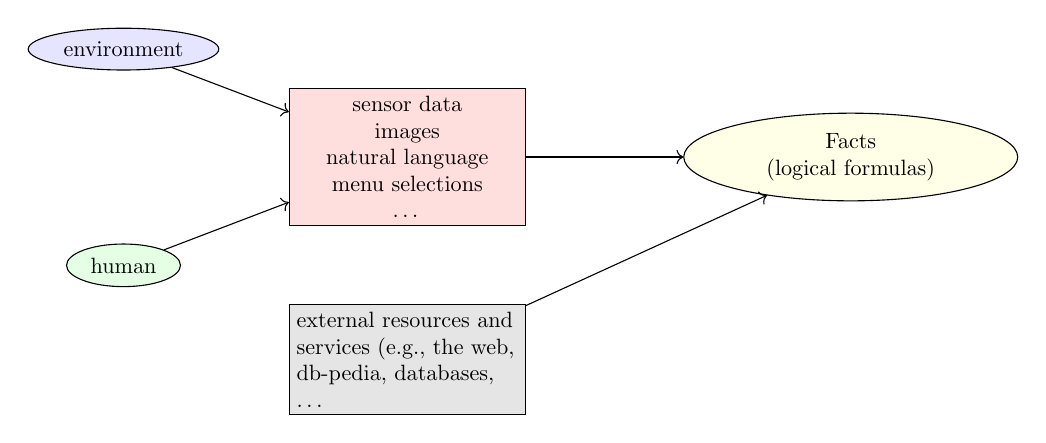
\begin{tikzpicture}[every node/.style={scale=.8}]
\node[ellipse,draw,fill=blue!10] (env) {environment}; 
\node[below = of env] (he) {};
\node[below = of he,ellipse,draw,fill=green!10] (hum) {human}; 
\node[draw,right =2 of he,fill=red!13,text width=10em,align=center]
(obs) {sensor data \\ images  \\ natural language \\ menu selections \\ \dots};
\node[text width = 10em,align=center,ellipse,draw,right=2 of
obs,fill=yellow!10] (facts) {Facts  \\ (logical formulas)};
\node[fill=gray!20,draw,below = of obs,text width = 10em] (web) 
{external resources and services (e.g., the
web, db-pedia, databases, \dots };
\draw[->] (env) -- (obs);
\draw[->] (hum) -- (obs);
\draw[->] (obs) -- (facts);
\draw[->] (web) -- (facts);
\end{tikzpicture}
\end{center}

\begin{definition}{Logical Model instantiation}
\label{def:logical-model-instantiation}
Model instantiation is the capability of transforming a (complex)
observation $o\in\Observations$ in either an entity or a formula 
in the language $\L$ of the logical model. 
\begin{align}
\logicalModelInstantiation:o\mapsto\text{$\L$-term}|\text{$\L$-formula}
\end{align}
\end{definition}




In most of the cases learning, this is done manually, but also
automatic methods as e.g., ontology population and inductive logic
programming, allow to learn models from a set of
data/observations. Update is usually obtained by adding or deleting or
modifying some formulas in the knowledge base.



\paragraph{Model update}
In updating/extending the model one has to pay attention to maintain
consistency at the price of minimal modification. The literature of
belief revision proposes a number of methods to solve this problem


\paragraph{Inference with the model}
Model inference is done via logicval inference, or rewriting, or
satistisfiabiliy or model checking.  For expressive logics the problem
of computing the logical consequence of a set of formulas is not
decidable. Therefore logical inference is guarantee to be complete
only on decidable fragments of the logic. For the other one have to
stay with incomplete or approximate inference engines.

\subsection{Probabilistic models}
\paragraph{Model definition:}
A probabilistic model \cite{murphy2012machine} is defined by a set of
random variables $X$ (i.e., a function that associates a value of the
outcome of an experiment). Random variables are split in two sets: the
observable variables $O$ and the hidden variables $H$. Each variable
is associated with a discrete or a continous domain. The second
component is a probabilistic distribution $P(X=x)$ over the set possible
values $x$ of the random variables. This funciton is called
\emph{probabilistic mass funciton} with $\sum_{x}P(x) = 1$, and
\emph{probabilistic density funciton} with $\int P(x) dx=1$.
Given a probabilistic model $P(X=x)$, and a value $o$ of the
observable variable, we are interested in computing the
$P(H=h\mid O=o)$, i.e., the conditional probability of the hidden
variables given the observations $o$. 

\paragraph{Model Schema Specification:}
The specification of the schema of a probabilistic model consists in
defining the set of random variables, their domain and their
(conditional) dependences. Usually, the set of variables are split in
two subset, the observables and the hidden variables.  Examples of
variables can be boolean variables that encodes propositions that are
true or false in the environment; integer variables that encode some
discrete quantity in the environment (e.g., how many friends has a
person), or continous variables that encode some continous measure in
the environment, e.g., the distance between the agent and the next
wall. The (in)dependency conditions between probablistic variables is
represented by a directed or undirected graph whose vertexes are the
random variables. That's why probabilistic model are often called
probabilistic graphical models \cite{koller2009probabilistic}.  The
second element of the schema of a probabilistic model is the shape of
the probability mass/density funciton of the join distribution of the
random variables. I.e., a parametric family of probabilistic
mass/density function.  A third component of the probabilistic model
schema, is a probability distribution over the parameter values. When
every parameter value is equiprobable, this information is
omitted. Usually thin part of the model schema is called \emph{prior},
as it represent some a priori knolwedge about the distribution of the
parameter values.

\paragraph{Model Instantiation}
In the probabilistic setting the model instantiation is usually called
\emph{model learning} or \emph{parameter estimation}. The main goal of
this phase is to find the (distribution over the) set of parameters
values that better fits the set of data/observations and, if it is
available some prior distribution over the parameters. For this one
can apply the Maximum Likelihood criteria, or the Maximum a posteriori
criteria, depending on the fact that a prior distribution on the
parameters is considered. There are three main methods that are used
to provide these estimation. We breafly summarize them in the
following assuming that the probablistic model is expressed by the
parametric pmf/pdf $P(D\mid\theta)$.

\begin{description}
\item[Maximum Likelihood (ML):] Given a set of observations $D$ we have
  the likelihood of the parameter values $\theta$, which s defined
  as $\theta^*=\argmax_{\theta}p(D\mid\theta)$. 
  In general, we would expect good choices of $\theta$ to assign high
  likelihood to the observed data. This suggests the maximum
  likelihood criterion: choose the parameter $\theta$ which maximizes
  $P(D\mid\theta)$ of the observed datas $D$.
  In some case this can be computed analytically,
  but in most of the cases when $P(D\mid\theta)$ is not a well known
  family, this is computed by approximated numerical optimization
  methods, similar to what is applied in neural networks and other
  numerical models. Notice that Maximum likelihood criteria does not
  require/uses information on the prior distribution over parameters
  and on the data.
\item[Bayesian posterior (B):] Bayesian estimation method do not compute a single
  values for the parameters, but rather a probablity distribution over
  the parameter values, starting from an initial probability
  distribution $P(\theta)$ on the parameters' values, known as the
  \emph{prior distribution} on the parameter values $\theta$. This
  distribution is supposed to encode agent's prior beliefs about the
  parameters before looking at the data. Once the agents observes $D$
  it's beliefs about $\theta$ might change, according to the Bayes
  rule.  In particular, the \emph{posterior distribution}
  $P(\theta\mid D)$ corresponds to our beliefs about the parameters
  after observing the data, which can be computed using Bayes’ Rule:
  $P(\theta\mid D) =\frac{P(D\mid\theta) P(\theta)}{\int
    P(D\mid\theta) d\theta}$. Therefore, this method does not do a
  single instantiation of the probabilistic model $P(D\mid\theta)$,
  but assigns a probability to all the possible instantiations of the
  model. 
\item[Maximum a posteriori (MAP):] This method instantiates the model with
  the value of $\theta$ that maximizes the posterior distribution
  $P(\theta\mid D)$. Ie $\theta^*=\argmax_{\theta}P(\theta\mid D)$. 
\end{description}

\paragraph{Model Update} 
Probabilistic model can be updated by changin the (distribution of)
parameter values, or updating the structure of the graphical model. An
update is usually the consequence of new (training) data available.
The update of the parameter (distribution) is performed by applying
the same method used for the model instantiation considering the
additional data. The update method depends from the specific method
used for the parameter estimation (Max Likelihood, Bayesian, Maximum a
Posteriori). At a high level we can think that this
update is
$$
\text{(ML,MAP):}\ \ \  \theta \stackrel{D}{\longrightarrow} \theta'
\ \ \ \ \ \ \ \ \ \ \ \
\text{(B)}\ \ \ P(\theta) \stackrel{D}{\longrightarrow} P'(\theta)
$$

\paragraph{Inference}
Given an instantiated mdoel over a set of variablex $X=O \cup H$ the
and an estimation of the parameters $\theta$, the problem of inference
is the problem of estimating the conditional probability of $P(H\mid
O,\theta)$, i.e., the probability the hidden variables $H$ given the
observations $O$. If we have a unique estimation of $\theta$ (obtained
by ML or MAP) the inference amounts in finding $P(H\mid
O,\theta^*)$. If instead we have a posterior distribution over
$\theta$ (obtained by Batesian estimation), we compute $\int_{\theta}
P(H\mid O,\theta)\cdot P(\theta) d\theta $.

\subsection{Real Function Models}

\paragraph{Model definition:}
Functional models are (real value) functions, (also called
\emph{predictors} \cite{deisenroth2020mathematics} Chapter 8.1) that,
given a particular input observation, encoded in a vector of $m$ real
value features, produces an output a prediction, which is a
real-valued vector. This can be written
as
$$
f :\R^m \longrightarrow \R^n
$$
The predictions of functional models are interpretable in different
ways depending on the specific application domain and task.
A \emph{classifier} is a model $f$  that classify the output vector
$\left<y_1,\dots,y_n\right>$ is interpreted as the probabilities that
the input observation is classified in the (disjoint) classes
$C_1,\dots,C_n$.  If $f$ is a regression model then it's output is
interpreted as an estimation/prediction of some unobservable quantity
that depends from the observations given in input (e.g., to predict
future stock market trend on the basis of historical data, the
distance of a robot from the objects on the basis of a pictures).
A \emph{data analysis} model $f$ can be used for clustering the data
or for embedding/encoding them in a low dimensional space.  
Examples of real function models are Neural Networks, Support Vector
Machines, Linear and Non linear regression models (linear, Linear,
Logistic, Polynomial, Stepwise, \dots). 

\paragraph{Model Schema Specification:}

The specification of the schema of a real function model consists in
three main components, that specifies the \emph{input features} to be
extracted from the observations, \emph{the shape of the function} and
its parameters, and the \emph{interpretation of the prediction} as in
terms of the task that the model is supposed to solve.
\begin{description}
\item[Design of input features]
Feature selection/definition is a key aspect. If observations are
already in the real field then features can be defined as real
functions on the observations. This can be done manually, or use
convolutional neural networks that are capable to automatically
extract features which are optimal for a certain task. When
observations are not in the real field, e.e., texts, or structured
information like relational data, one possibility is to use embeddings
i.e., functions that are capable to map discrete structured data into
real field, perserving similarity. E.g., one of the most famous
embeddings used for text is BERT \cite{devlin2018bert}.

\item[Specify the structure of $f$] The core of a real function model
  is the parametric family from which the function is selected. The
  two key components that one has to define are the set of parameters
  (as in the case of probabilistic models) and the shape of the
  function. For instance, the structure of linear models are
  $f(x) = W\cdot x + B$ wehre $W$ is an $m\times n$ matrix of
  parameters and $B$ is a vector of $m$-parameters, and $f$ is defined
  as an affine transformation on the input features $x$.  Deep neural
  networks defines much more complex structures of a function, but the
  principle remain the same. In most of the case these design is done
  manually, and currently there is not a comprehensive study of the
  advantage/disadvantage of choosing a structure or the other. Some
  study on the relationship on the network architecture and their
  performance in different tasks has beed done recently, see for
  instance \cite{lathuiliere2019comprehensive,cortes2017adanet}.
  There are however some studies on automatic ways to overcome the
  problem of choosing the optimal network architecture
  \cite{saxena2016convolutional,xie2017genetic}.  Overall, there is
  very little guidance on the plethora of design choices and
  hyper-parameter settings for deep learning architectures.

\item[Output interpretation]
  The output of a functional model is a vector in $\R^m$ and the
  artificial agent should be provided with a way to use this output in
  order to take decisions and actions. This interpretation is also
  necessary in order to evaluate the correctness of the model, i.e.,
  if it performs correct or wrong predictions. This interpretation is
  encoded in the so called \emph{loss function} that provides a measure
  (i.e., a real number) of quality of the performance of the model by
  measuring how far is the prediction of the model from the correct
  one (i.e., the error ration of the model). In classifiers for
  instance the loss function measures the mis-classification rate,
  while in regression it measures the distance between the correct
  answer and the predicted answer. In models for clustering or
  encoding the loss measures the quality of the clustering. 
\end{description}

\paragraph{Model Instantiation}
The instantiation of a real function model schema consists in
finding the parameters values of the model that minimizes the loss
function computed on a set of data provided in input. This is quite
similar to the criteria of maximum likelihood applied to instantiate
the probabilistic models. In case of supervised learning, where we
have a set of pairs input output the optimization is defined as
$$
\argmin_{\theta}\mathcal{L}(y^{(1)},\dots,y^{(k)}, f(x^{(1)}\mid\theta),\dots,f(x^{(k)}\mid\theta))
$$
where $\mathcal{L}$ is the function that compares the correct
predictions $y^{(i)}$ with the predictions done by the model
$f(x^{(i)}\mid\theta)$ instantiated with the parameter values
$\theta$.
In case of data analysis algorithms, the loss function is defined only
w.r.t., the data input (this methods are usually called unsupervised
learning). The learning in this case is defined as follows: 
$$
\argmin_{\theta}\mathcal{L}(f(x^{(1)}\mid\theta),\dots,f(x^{(k)}\mid\theta))
$$
In both cases the instantiation is done with respect to a set of data
that are provided in input. The result of the learning depends in a
substantial way on the quality and quantity of data provided in input
for training. 

\paragraph{Inference}
Inference in functional models consists in just computing the value of
the function on a given input i.e.,
$$
x \mapsto f(x)
$$
\paragraph{Model update}
Model update when some new data become available mainly happens by
reinstantiating he model, considering the loss with respect to a
combination of the ``old data'' and the ``new data''. Such a
combination can be just the union, or some weighted combination.

\subsection{Action Models}

  \paragraph{Model definition}
  \emph{Action models} specifies the expected advantage an agent
  can obtain in following a certain policy (= action selection
  strategy). This category of models contains planning models,
  Markov Decision Processes, game theoretic models, and action preference
  models. In the literature there are many different types of action
  models, and we don't try to summarize them in a single definiton. We
  rather report below what are the basic components of an action
  model.

  \begin{description}
  \item[State space] a set of states in which the agent can be. This set could be
    the set of all the observations/perceptions of the agent (in case
    of full observable models) or a set of latent states which depends
    from the observations. 
  \item[Action space] a set of actions that can be executed by the agent. 
  \item[Transition relation] a description of the preconditions of the actions (when they
    are possible) and the effects of the actions. These effects can be
    deterministic, or non deterministic. This component in some models
    is not strictly necessary.
  \item[Policy or plan] a policy, i.e. a function that for every state provides a
    (probability distribution of) action(s) that should be executed.
  \item[Goal] the specification of one or more alternative situations
    that the agent should achieve. Or the specification of a
    preference relation (partial order) on the possible outcomes. 
  \end{description}
  
  \paragraph{Model schema specification}
  The definiton of the model schema fixes the set of actions, and the
  set of states. Actions can be specified as atomic actions (e.g.,
  turn-left, turn-right, \dots) or with some argument (e.g., go
  forward of $1m.$, turn of $45^\circ$, move block 1 on top of block
  2). The set of states, can be specified explicitly by enumerating
  all the states or by providing a set of state variables
  $V_1,\dots,V_n$ that take values in domains $D_1,\dots,D_n$ and
  define the set of states as a proper subset of $\times_{i=1}^nD_i$
  by means of constraints. The planning and the robotic communities
  have developed a number of languages for expressing actions schemata
  see \cite{nakawala2018approaches}.  In the area of reinforcement
  learning states and actions are often specified explicitly but there
  are examples of languages for more structural specification see
  e.g., \cite{jothimurugan2019composable,li2017reinforcement}.  In the
  area of game theory, a game schema can be described either
  explicitly, by describing the set of states, the type of actions
  (that each agent can perform) and their effects, or one can use a
  specification language as for instance Game Description Language
  \cite{thielscher2011general,jiang2016epistemic,kowalski2016towards}.

  \paragraph{Model Instantiation}
  
  \paragraph{Model Inference}

 \begin{itemize}
  \item Reinforcement learning:  Reward function $\rightarrow$ optimal policy

  \item planning: goal $\rightarrow$ optimal plan

  \item game theory: utility function $\rightarrow$ equilibrium 
  \end{itemize}
  \paragraph{Model update}

  \subsubsection{Optimization models}
  Optimization models \cite{nocedal2006numerical}
  represents the world in terms of a set of
  real functions $f_i:\R^m \rightarrow \R$. over $n$ real variables
  $x_1,\dots,x_n$. Observations on the real world are mapped into
  constraints on the values of such a variables, e.g., the observation
  that the temperature is $21^\circ$ with an erro of $0.1^\circ$, is
  represented by the constraint $20.9\leq x_{temp}\leq 21.1$. Other
  variables are in control of the agents who can operate in order to
  set their values. These variables also corresponds to some
  proposition about the state of the world. The environment in which
  the agent operates, should also have a number of physical
  constraints, which are also represented in terms of constraints on
  the values of observable and control variables. 

  \paragraph{Definition}
  An optimization model consists in a 
  function that have to be minimized relative to some set, representing a range of choices
  available in a certain situation. The function allows comparison
  of the different choices for determining which might be best.  More
  formally we define the optimization model in terms of
  \begin{itemize}
  \item a funciton $f(x):\R^n\longrightarrow R$
  \item a set of equality constraint $\{g_i(x) \geq 0\}_{i\in EC}$ where
    $g_i:R^n\longrightarrow R$.
  \item a set of constraint $\{h_i(x) = 0\}_{i\in IC}^m$ where
    $h_i:R^n\longrightarrow R$. 
  \end{itemize}
  The set $S=\{x\in\R^{n}\mid g_i(x) \geq 0, \mbox{ and } h_j(x)=0\}$
  is the set of ``admitted solutions'', in other words the space of
  decisions, from which the agent have to select the optimal one. 
  
  \paragraph{Model Schema Specification:}
  Optimization model schemata are well defined they are described
  along two dimensions. The domain of decision variables, namely
  discrete or continous, and the presence of constraints, namely
  constrained or unconstrained. A third dimension are the family of
  functions to be optimized and the constraint functions: namely,
  linear or non linear functions. Furthermore the constraint region
  can be conves or non-convex. 

  \paragraph{Model Learning/Instantiation}
  Model specification is the process of identifying the objective
  funciton $f(x)$, the set of unknown variables and the constraints
  for a given problem Construction of an appropriate model is the
  first step---sometimes the most important step---in the optimization
  process.
          
  \paragraph{Inference with the model}
  Inference amounts in running some optimization algorithm that find
  an (approximate) solution of the optimizaiton model with respect  to
  some observations. I.e., to solve the problem
  $$
  x^* = \argmax_x f(x)  \ \ \ \ \ \ \ \ \mbox{under the constraint
    $x\in S$. }
    $$
  There is a large literature of optimization algorithms, which are
  general purpose or domain specific. They can provide caertain or
  approximate answer. They can return global or local optimum. 
    
  \paragraph{Updating the model}
  Optimization model can be updated by adding or deliting some
  constraint or by modifying the objective function. 


\section{Explainable, Verifiable and Collaborative AI systems} 

\subsection{Explainable AI} Explanable AI is the problem of providing
explanations to humans about some inference done by AI agent with it's
model. Depending on the model different explanations are possible:
For a survey of XAI see \cite{arrieta2020explainable}

A specific form of explanation is \emph{contrastive explanation}
\cite{miller2018contrastive} provides a formal framework for
contrastive explanation by extending \emph{structural causal models}
\cite{halpern2005causes1}.  The work define the notion of
\emph{contrastive explanation}, 
that is the explanation of an event relative to some contrast case, as
for instances explanations for questions like ``Why P rather than
Q?''. The proposed formalisation is intended to be general and
applicable to a wide rante of AI models.

\begin{description}
\item[Explanations of an inference in logical model] Though
  explanation are manly advocated for inference performed by deep
  neural networks, explanations are also necessary for inference
  performed in logical systems, in order to reach human centered
  artificial intelligence.

  Consider for instance the situation were an
  agent uses a SAT solver for answering the question $\phi$ posed on a
  knowledge base $K$. Suppose that $K\models\phi$. This implies that
  the agent will provide a positive (or negative) answer. But what
  about the explanation of such an answer?  The Solver will show that
  $K\cup\{\neg \phi\}$ is not satisfiable and for doing this it will
  search all the truth assignments without finding one that satisfies
  $K$ and $\neg\phi$. Showing the trace of the search would not
  constitute a good explanation. Alternatively the agent could provide
  a minimal set $K''subset K$ from which is it spossible to derive
  $\phi$ (i.e., to show that $K'\cup\{\neg \phi\}$ is
  inconsistent). Still the size of $K'$ might be very big and not
  understandable by a human. Furthermore, the encoding of the model in
  the set of axioms $K$ should not be very easy to read by a
  human. This means that an explanations should also contain the
  intuitive meaning of the langauge used to formula the knowledge base
  $K$. When the answer is negative i.e., if $K\not\models\phi$, then
  an explanation could be given in terms of a counter-model, i.e., an
  assignment that makes $K$ true and $\phi$ false. This is certainly
  mre readable than the previous case, but still the meaning of the
  axioms in $K$ should be conveyed to the human.

  A second method used for doing inference in logical model is to
  search for a deduction from the set of observations $O$ to the query
  $\phi$ (or $\neg\phi$), or viceversa find a proof from $\phi$ to $O$
  or from $\neg\phi$ to $O$. This is the case of explanation.
  In both cases an explanation is a sequence or a directed graph of
  formulas with $O$ and $\phi$ (or $\neg\phi$) at the extreme.

  In all the cases explanation is provided in terms of logical
  symbols. Therefore, to be understandable by humans, humans should be
  able to ascribe a meaning to these symbols. E.g, an explanation that
  contains the symbo $p124$ is probably not satisfactory. 
  
\item[Explanations of inference in probabilistic model] One of the
  basic inference task in probabilistic model is called \emph{Most
    Probable Explanation (MPE)}. MPE is the problem of finding a
  complete assignment of values to a set of variables that has the maximum
  likelihood given some variables that are instantiated with some
  observations. Formally the MPE is the following problem:
  $$
  \argmax_{x}Pr(X=x\mid E=e)
  $$
  where $E$ and $X$ are disjoint set of random variables. Intuitively
  the solution of the MPE is a value of $X$ that better explains the
  observation $e$. This is a rather crude explanation, that does not
  provide any rational argument behind the final decision of the
  model. A more sophisticated notion of explanation of the inference
  in a statistical model is offered by considering causal models
  \cite{pearl2009causality}, interventions, and counterfactuals.
  \cite{chajewska2013defining,halpern2005causes1,halpern2005causes2,%
    sprenger2018foundations,peters2017elements}.  In this case
  explanation are defined as \dots (TO BE FINISHED)

\item[Explanations of an inference in real function model]
  The massive interest on explainability has surged due to the success
  of deep neural network. Various form of explanations has been
  proposed for the conclusion obtained from a DNN.  A very general
  definition of explanation of the decision of a real function can be
  defined with the help of causal models.
  In particular, in \cite{chattopadhyay2019neural} a deep neural
  network is seen as a Structural Causal Model \cite{pearl2009causality}

  An alternative approach, which consider only the imput/output pair
  of the model is by determining the contribution of each single imput
  feature to the final prediction by using additive feature
  attributions. 

  \begin{definition}[Additive feature attributions]
      Suppose $f:\mathcal{X} \rightarrow\mathbb{R}$
is a model mapping an $M$-dimensional feature space $\mathcal{X}$ to realvalued
predictions. Additive feature attributions for $f(\mathbf{x})$ at
input $\mathbf{x}=(x_1,\dots,x_M)\in\mathcal{X}$, 
comprise of a reference (or baseline) attribution $\phi_0$ and a set
of feature attributions $\phi_1,\dots,\phi_n$ such that $f(\mathbf{x}) =
\phi_0+\sum_{i=1}^M\phi_i$. 
\end{definition}
According to the previous definition $\phi_i$ is the contribution of
the feature $x_i$ to the decition $f(\mathbf{x})$. 


  
\item[Explanations of an inference in action model] Action models
  include planning model, reinforcement learning models and game
  theoretic models. For each of the type of model a specific notion of
  explanations has been developed. In the following we quickly analyse
  them.
  
  \paragraph{Explanations in Planning} The approaches and the
  challenges of explanation in planning are described in
  \cite{chakraborti2020emerging}, which defines the different forms of 
  \emph{explanations of a plan or a policy as a solution of a given
    planning problem}. A planning problem is composed of a planning
  domain and a desired property (goal + optimality condition, \dots).
  The solution of a planning problem is a plan or more generally a
  policy i.e., a function $\pi: S\rightarrow A$ that select the
  actions to execute if the agent is in a specific state.
  \begin{align}
    \label{eq:plannin-decision}
  \Pi, \pi\models \tau
  \end{align}
  means that, $\tau$ can be achieved by following the policy $\pi$
  in the planning domain $\Pi$. 
  An explanation of the decision \eqref{eq:plannin-decision} 
  is an artifact $\mathcal{E}$ ``understandable by the explanee'' such that
  $$
  \mathcal{E},\pi\models_u\tau 
  \mbox{ and }
  \mathcal{E},\pi'\not\models_u\tau
  \mbox{ 
    for all $\pi'$ different from $\pi$.}
  $$
  The content of the
  explanation $\mathcal{E}$ can vary greatly depending on the needs of
  the explainee.
  
  \paragraph{Explainable reinforcement learning}
  For a survey in explanations in Reinforcement Learning see
  \cite{puiutta2020explainable}. We report here two approaches that
  provide a clear and formal definition of explanation in
  reinforcement learning. 
  
    \cite{sequeira2019interestingness} proposes an explainable reinforcement learning
    (XRL) framework that analyzes an agent’s history of interaction
    with the environment to extract interestingness elements that help
    explain its behavior. In a nutshell the explanation of the
    behavious of the agent is provided in terms of four aggregations
    values about the interaction the agent has with the enviroment.
    In particular suppose that the agent interaction is the following
    sequence
    $$
    t= z_0,a_1,r_1,z_1,a_2,r_2,\dots z_{n-1},a_n,r_n,z_n
    $$
    they propose to ``explain'' the behavious of the agent in terms of
    Frequency, Transition Value, Execution Certainty, Sequences, which
    can be computed starting from the trace $t$.

    From the same data (trace $t$) \cite{madumal2019explainable} learn
    a causal model as defined in \cite{halpern2005causes1} from which
    they are capable to provide counterfactual explanations of why an
    action has (not) been executed in a certain state $s$.  The causal
    model is a DAG where state variables are linked trough actions,
    intuitively $X\stackrel{\rightarrow}{A} Y$ where $X$, and $Y$ are
    state variables and $A$ an action, suggests that the value of $Y$
    after the execution of $A$ depends on the value of $X$.  The
    leaves nodes of the DAG correspond to the rewards.  The
    explanation of ``why the action $a$ in state $s$'' is given in
    terms of the values of the variables entering in the action $A$,
    and the values of the variables entering in the final reward.  The
    explanation of ``why not action $b$ in state $s$'' is given in
    terms of conterfactual explanation. I.e., by comparing the
    explanation of $a$ in $s$ and the explanation of $b$ in $s$.
    
    \paragraph{Explanation in Game theory}
    No specific method has been found for explaining decisions taken by
    game theoretic models. Instead game theoretic approaches have been
    used to provide explanations in other models. 
    \cite{merrick2019explanation} proposes a general game theoretic
    method to generate explanations based on additive feature
    attributions.

  \item[Explanations of an inference in optimization model] One of the
    most important application domain of optimization is
    scheduling. Explanation is scheduling has been defined in
    \cite{vcyras2019argumentation} via argumentation.  The aurthors
    formally define argumentative explanations as to why a given
    schedule is not ‘good’. We can define the framework very
    abstractly as follows; Let $M$ be a makespan problem and $S$ be an
    optimal and feasible schedule for $M$. Then we write
    $$
    M,S \models O \wedge F \wedge D
    $$
    where $O$ is a formula expressing the optimality condition w.r.t.,
    a partial order $<_S$ on the set of schedules. 
    $F$ is a formula expressing the feasibility condition imposed in $M$
    and $D$ if a formula expressing the desiderata (from the user),
    i.e., a subset of schedules. 
    The proposed approach provide explanations for 
    $$
    M,S\not\models O 
    $$
    by finding a schedule $S'\neq S$ with better perfornmance w.r.t.,
    $S$.
    The explanation of 
    $$
    M,S\not\models F
    $$
    By finding the minimal $M',S'\subseteq M,S$ such that
    $M',S'\not\models F$. Similarly, the explanation of
    $$
    M,S\not\models D
    $$
    is provided by finding a minimal subpart of $S'\subseteq S$
    such that for all $S'\not\subseteq S''$ for all $S''\in O$> 

    {\color{red}FROM MICHELE \tt

      1) Visto che la maggior parte dei sistemi di ottimizzazione si
      basano su modelli definiti da esperti, il problema della
      spiegazione è decisamente meno sentito.

      Un esperto non ha in generale difficoltà ad interpretare una
      soluzione. Anche nel caso il modello sia un po’ convoluto
      (capita in SAT e MILP in particolare), è generalmente facile
      presentare una sua soluzione in termini naturali per un esperto.

      2) Parecchio lavoro è stato dedicato allo spiegare l’ottimalità
      o l’infeasibility (i.e. perché una certa soluzione è ottima, o
      cosa la rende infeasible).

      Questi temi però non li trovi associati al termine
      “explainability”, perché è nato molto più tardi. Si parla invece
      di:

      - Irreducible Infeasible Sets (in MILP)
      
      - Conflicts (in CP e SAT)
      
      - reduced costs (come  prova di ottimalità in LP)
      
      - Minimal Critical Sets (in scheduling)
      

      Addirittura c’è gente che usa questi approcci per spiegare le
      predizioni delle deep network (dopo averle tradotte in modelli
      simbolici).

In sintesi:

1) Il temine “explainability” non è di sicuro molto usato in contesto di ottimizzazione
2) Il problema di  spiegare modelli e soluzioni non è molto sentito, se non in alcuni contesti specifici (vedi sopra).
3) Detto questo, qualcosa potenzialmente da fare ci sarebbe. Per esempio, i vari approcci per l’individuazione di conflitti etc. hanno tradizionalmente una finalità tecnica: i  conflitti estratti sono utili per i solver, ma non necessariamente chiari per un  essere umano.
    }
  \end{description}
  
\subsection{Verifying AI models}

\rb{Should we only aim for covering deductive software verification?} % possibilities below:

%deductive verification
%model checking
%general proof assistants
%correctness by construction
%SMT solvers
%runtime verification
%software testing
%coverage criteria for testing
%static analysis
%dynamic analysis
%...
%formidable challenges lie ahead with respect to verifiable AI...!



\todo{add relations between safety and liveness properties of
  different AI models \dots Raul}
  
% single-agent (the AI agent) and non-deterministic environments, sensors and actuators. This is what we have also in the “onion”, i.e., observations (produced by sensors) and actions (Produced by actuators); if humans are taken into account. They act independently from the artificial agent, and therefore they are a source of indeterminism in the environment. Explain how this leads us into safety and liveness properties, and notions of fairness; temporal logics may be applied as a means to specify such requirements. humans interact with the environment and with the agent, in a feedback loop.

Verifiable AI consists of the set of methods, techniques and tools
that support checking key properties of an AI system or a larger
system that includes AI as one or more key components.  In this part
we concentrate only in the verification of the AI component of a
system, i.e., the AI model. In general we can distinguish between
functional and non functional requirements. Non functional
requirements specifies how the sistem should be rather than what it
should do. Since we consider `abstract AI models'' we focus on
verification of functional requirements on how the model and behaves
in all it's phases. 
  
 \begin{description}
 \item[Verifying logical models] The behavior of a logical system is
   encoded in the logic itself, and once one is able to encode the
   conditions that the system should comply in terms of a set of pairs
   of formulas $\left<\phi_o,\phi_a\right>$ where $\phi_o$ are the
   properties of the input observation and $\phi_a$ encodes the
   property of the decision/action taken by the system, then the one
   can check if 
   $$
   M_L, \phi_o \models \phi_a
   $$
   and it will be guaranteed that whenever the model receives in input
   an observation that satisfies $\phi_o$, (i.e., $O\models \phi_o$)
   then the output generated will necessarily be an action that
   satisfies (or is consistent with) $\phi_a$.
   
 \item[Verifying probabilistic models]
   Formal verification of bayesian networks \cite{pmlr-v72-shih18a}
   Probabilistic model checking \cite{kwiatkowska2018probabilistic}

 \item[Verifying numerical models] According to
   \cite{kohli2019towards}, there are three main groups of
   verification tasks Adversarial Testing, Robust learning, and Formal
   Verification. There are many works in the area of formal
   verification of neural networks and other numerical model.
   However, one of the most important element of the models which are
   learned via supervision, are the properties of the training data.
   Important aspects to be verified are also the fact that the system
   don't use certain critical data to do the prediction.

   \cite{narodytska2018formal} discusses a set of interesting
   properties of neural network, including properties that relate
   inputs and outputs of the network, e.g. robustness and
   invertibility, and properties that relate two networks, like
   network equivalence. For instance one property of the neural
   network is global $\epsilon$-robustness. 

   A feedforward neural network $f:\R^n\rightarrow \{0,1\}^m$ is
   globally $\epsilon$-robust if for any $x,\tau\in\R^n$ with
   $||\tau||_{\infty} \leq \epsilon$, $f(x+\tau)=f(x)$. 
   
 \item[Verifying action models]
   model checking \cite{clarke2018introduction} and
   probabilistic model checking \cite{kwiatkowska2018probabilistic}
   Formal verification of reinforcement learning
   \cite{van2017challenges}
   
 \item[Verifying optimization models]
   
\end{description}

\subsection{Co.AI}
\begin{description}
\item[Collaboration with agents with logical models]
\item[Collaboration with agents with probabilistic models]
\item[Collaboration with agents with numerical models]
\item[Collaboration with agents with action models]
\item[Collaboration with agents with optimization models]    
\end{description}

\section{Related work}

\subsection{Human centered AI frameworks} 
\todo[inline]{add related work to \cite{wei2019toward}}
\todo[inline]{Add related work with Humane AI project}

\subsection{Ontologies for Human Centered Artificial Intelligence} 

\todo{maybe we can add some related work with the effort done in AI4EU
  and other projects to create an ontology for Human Centered
  Artificial Intelligence} 

AI4EU has developed an ontology that is used to describe the AI
resources availeble on the AI4EU platform \cite{ai4eu-D3.4}. 
The main concept introduced by the AI4EU ontology is the one of \emph{AI
  resource}. According to the deliverable an AI resource is:

\begin{quote}\it
\dots any entity that can be used for obtaining knowledge or
technology around AI. This can be specialized by various subclasses
that conceptualise different types of technology e.g., Dataset,
Software, Hardware, Ontology, etc. This can be specialized by various
subclasses that conceptualise different types of technology e.g.,
Dataset, Software, Hardware, Ontology, etc.
\end{quote}

There are also other attemps towards an ontology for Artificial
Intelligent Agent. One example is \cite{hawley2019challenges}. 
\todo{LS: Check \cite{hawley2019challenges} and see if there is something interesting} 

We can think that the main topic of dicussion of this paper is an
attempts to organize the subclasses of AI resources according to a
certain set of creatiria. In this sense what we have done in this
paper is orthogonal w.r.t. to the ontology defined in
\cite{ai4eu-D3}. A possible intersection between the vision
proposed in this paper, and the AI4EU ontology concerns also the
\emph{technical category}
tribute of AI-resources \texttt{AI\_Technical\_Category}. The possible
values of such an attributes are labels that refers to concepts
defined in this paper. For instance the labels ``computational logic'',
``deep learning'', ``constraints and sat'', ``probabilistic models'',
can be associated to an AI-resources that implements a logical model,
a functional model, a constrained modle and a probabilistic model,
respectively.

Apart from such a categorization it seems that the main concepts
introduced in this paper provides a description of AI-resources which
is complementary to the information provided by the AI4EU ontology.
Developing an ontology for AI-resources according to the decription of
this paper would be an interesting task and it could integrated with
the AI4EU ontology in order to complement the description of
AI-resources 

%%% Local Variables:
%%% mode: latex
%%% TeX-master: "main"
%%% End:

\section{Conclusions}



\bibliographystyle{abbrv}
\bibliography{biblio}
\end{document}
